CRDT have some caracteristic:
\begin{itemize}
	\item The concurrent operations are natively commutative.
	\item The document is a linear sequence of elements.
	\item A unic position identifier.
\end{itemize}~

For the experiments, they select differents algorithms for generating the unic position identifier:
\begin{itemize}
	\item Logoot
	\item RGA
	\item WOOT
	\item WOOTO
	\item WOOTH
\end{itemize}

Figure \ref{fig:worst} p.\pageref{fig:worst} (with R the number of replicas and by H the number of operations on the document) shows the theoretical evaluation of this differents algorithms. RGA and Logoot have the bests results.

\begin{figure}[h]
  \center
  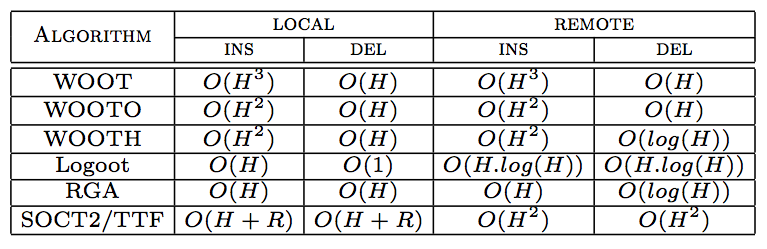
\includegraphics[width=0.7\textwidth]{includes/worst.png}
  \caption{Worst-case time-complexity analysis}
  \label{fig:worst}
\end{figure}


But this is just theoretical. The equip of the paper designed real-time peer-to-peer collaborations in order to obtain there logs and apply them on the algorithms. For real applications, two experiments and severals groups have been mades:
\begin{itemize}
	\item 3 grups have to do there semester report only using the collaborating editor during one and a half hours:
		\begin{itemize}
			\item 2 grups of 4 students.
			\item 1 grup of 5 students.
		\end{itemize}
	\item 9 grups of 2 students have to translate an episode of \emph{The Big Bang Theory}
\end{itemize}~

Figure \ref{fig:operations} p.\pageref{fig:operations} shows the total number of users/character operations:
\begin{itemize}
	\item A user operation is adding/deleting letters or grups (copy/past).
	\item A character operaton is the transformation of each user operation into a character operation (for example, copy/past "alma" are the character operations: \begin{itemize}
					\item adding 'a' at space 0
					\item adding 'l' at space 1
					\item ...
				\end{itemize}
\end{itemize}~

\begin{figure}[h]
  \center
  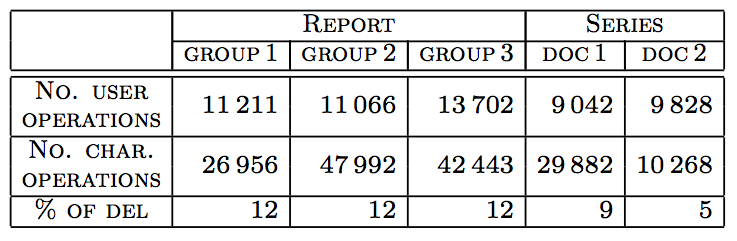
\includegraphics[width=0.7\textwidth]{includes/operations.png}
  \caption{Total number of user/character operations}
  \label{fig:operations}
\end{figure}

All the algorithms have been runned 10 times with same datas and sames conditions. Figures \ref{fig:users_operations_1t_big} and \ref{fig:users_operations_2g_report} p.\pageref{fig:users_operations_2g_report} shows the total number of users operations.

%\begin{figure}
%	\center
%  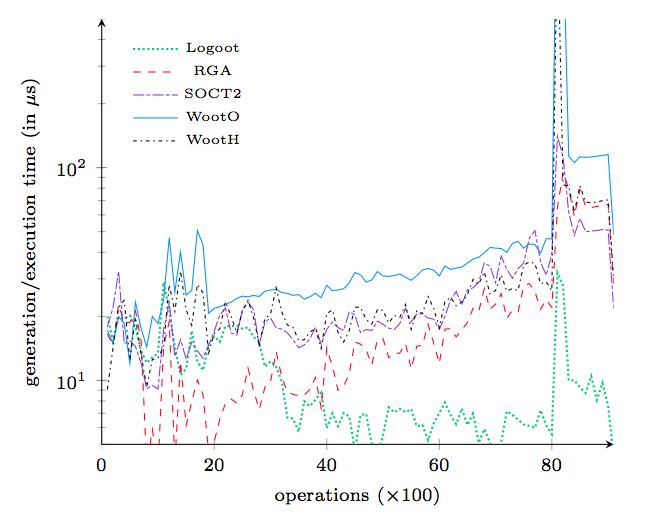
\includegraphics[width=0.6\textwidth]{includes/users_operations_1t_big.png}
%  \caption{User operation execution times - 1st series}
%  \label{fig:users_operations_1t_big}
%\end{figure}  
%\begin{figure}
%	\center
%  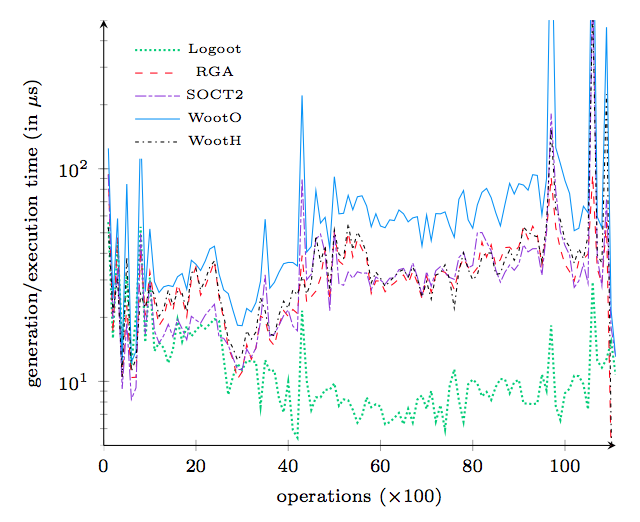
\includegraphics[width=0.6\textwidth]{includes/users_operations_2g_report.png}
%  \caption{User operation execution times - 2nd group
%report}
%  \label{fig:users_operations_2g_report}
%\end{figure}

\begin{figure}
\begin{minipage}{.50\linewidth}
    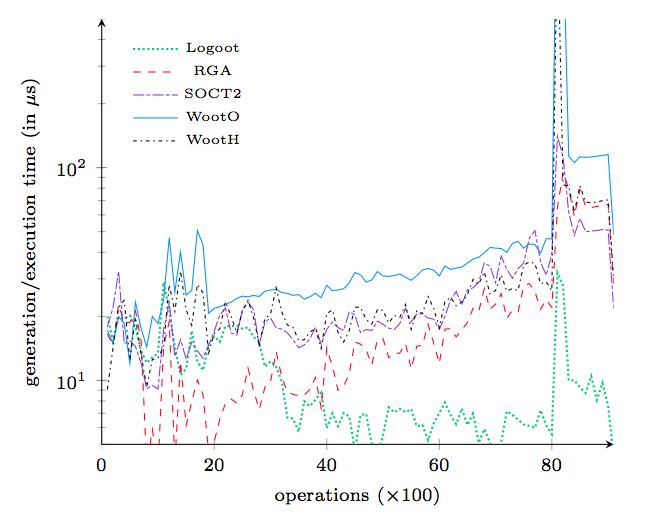
\includegraphics[width=1.2\textwidth]{includes/users_operations_1t_big.png}
  	\caption{User operation execution times - 1st series}
  	\label{fig:users_operations_1t_big}
\end{minipage} \hfill
\begin{minipage}{0.50\linewidth}
  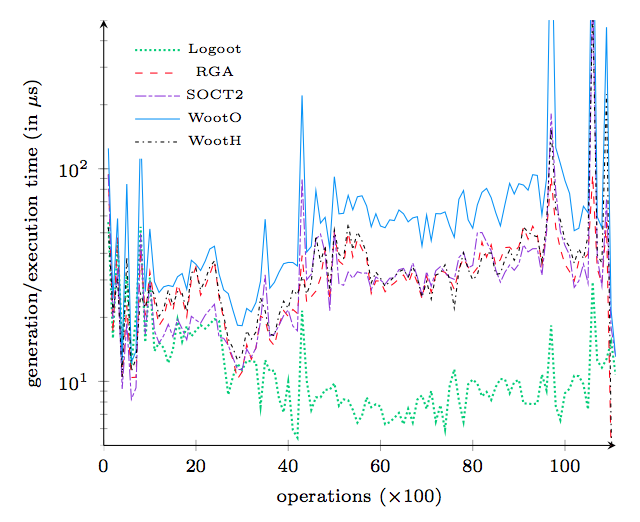
\includegraphics[width=1.2\textwidth]{includes/users_operations_2g_report.png}
  \caption{User operation execution times - 2nd group
report}
  \label{fig:users_operations_2g_report}
  \end{minipage} \hfill
\end{figure}

The increases are due to insert or delete a large group of characters on the document. All the algorithms decrease over the time because of the size of the document (the unique identifier is bigger when there is a lot of operations) but logoot decrease slowly than the others.\\

\begin{figure}
\begin{minipage}{.50\linewidth}
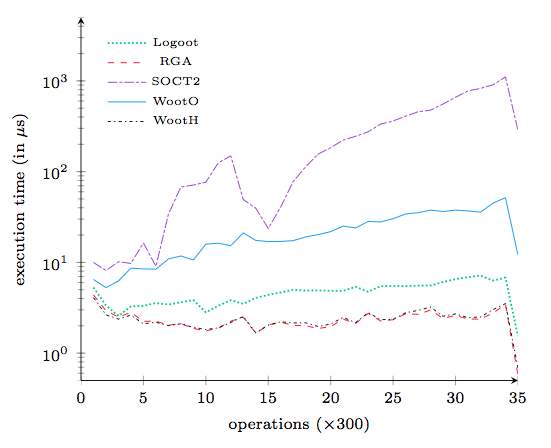
\includegraphics[width=1.2\textwidth]{includes/characters_operations_1t_big.png}
  \caption{Character operation execution times - 2nd
series}
  \label{fig:characters_operations_1t_big}
\end{minipage} \hfill
\begin{minipage}{0.50\linewidth}
  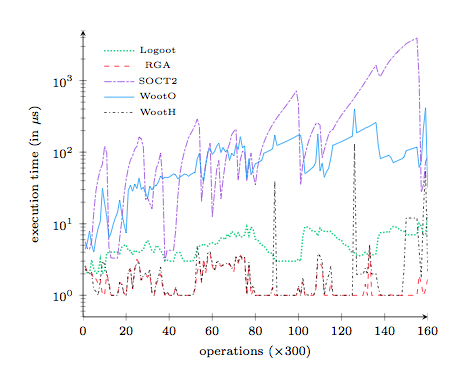
\includegraphics[width=1.2\textwidth]{includes/characters_operations_2g_report.png}
  \caption{Character operation execution times - 2nd
group report}
  \label{fig:characters_operations_2g_report}
  \end{minipage} \hfill
\end{figure}